\documentclass{beamer}
\usetheme{Madrid}
\colorlet{beamer@blendedblue}{green!40!black}
\setbeamertemplate{caption}[numbered]
\usepackage{amssymb, amsmath, amsthm}
\usepackage{physics, siunitx}
\usepackage{float, subcaption, graphicx}
\usepackage{hyperref}

\title{Introduction to Dense Plasma Focus (DPF)}
\author{Hunt Feng\inst{1}}
\institute[Usask]
{
	\inst{1}%
	Department of Physics and Engineering Physics\\
	University of Saskatchewan
}
\date{\today}

%%%%%%%%%%%%%%%%%%%%
% section page 
%%%%%%%%%%%%%%%%%%%%
\AtBeginSection[]
{
	\begin{frame}{Outline of Presentation}
		\tableofcontents[currentsection]
	\end{frame}
}

\begin{document}
%%%%%%%%%%%%%%%%%%%%
% title and TOC
%%%%%%%%%%%%%%%%%%%%
\maketitle
\begin{frame}{Outline of Presentation}
	\tableofcontents
\end{frame}

%%%%%%%%%%%%%%%%%%%%
% contents 
%%%%%%%%%%%%%%%%%%%%
\section{Pinch Effect}
\begin{frame} {Z-Pinch}
    \begin{itemize}
        \item Current generates $B$ field in $\theta$ direction.
        \item $\mathbf{J\times B}$ points radially inward.
    \end{itemize}
    \begin{figure}
        \centering
        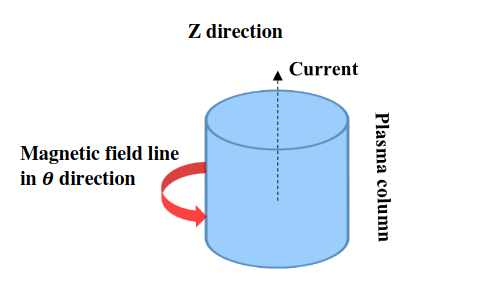
\includegraphics[width=0.7\textwidth]{figures/z-pinch.png}
        \caption{A Z-pinch in cylindrical coordinates. \cite{behbahani_2017_enhancement}}
        \label{fig:z-pinch}
    \end{figure}
\end{frame}

\begin{frame} {$\theta$-Pinch}
    \begin{itemize}
        \item Plasma current generates $B$ field in z direction.
        \item Current in primary loop together with $B$ field creates radially inward force.
    \end{itemize}
    \begin{figure}
        \centering
        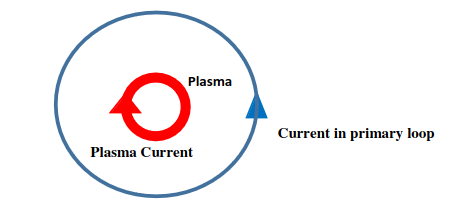
\includegraphics[width=0.7\textwidth]{figures/theta-pinch.png}
        \caption{A Schematic of theta pinch configuration. \cite{behbahani_2017_enhancement}}
        \label{fig:theta-pinch}
    \end{figure}
\end{frame}

\begin{frame} {$X$-Pinch}
    \begin{figure}
        \centering
        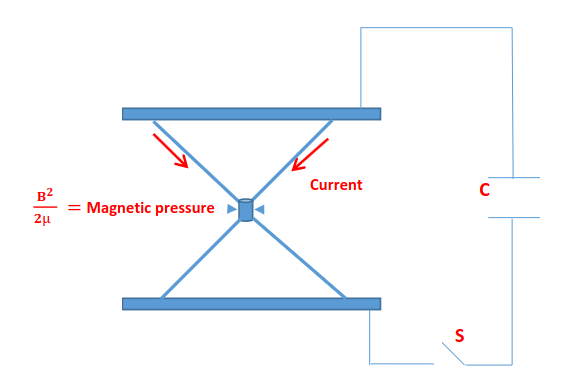
\includegraphics[width=0.7\textwidth]{figures/x-pinch.png}
        \caption{The configuration of an X-pinch device. \cite{behbahani_2017_enhancement}}
        \label{fig:x-pinch}
    \end{figure}
\end{frame}
\section{Dense Plasma Focus}
\begin{frame} {Plasma Focus Device}
    \begin{figure}
        \centering
        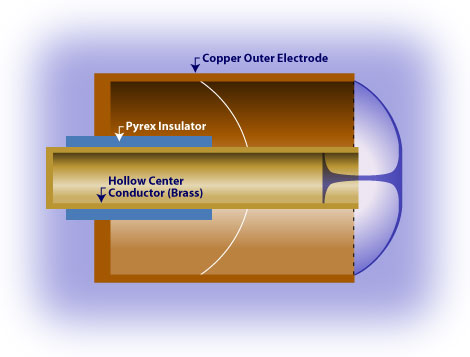
\includegraphics[width=0.7\textwidth]{figures/dfp-device.jpg}
        \caption{Plasma focus device (schematic). Source \cite{plasmauniverse_dense_plasma}}
        \label{fig:dfp-device}
    \end{figure}
\end{frame}

\begin{frame} {How It Works}
    \begin{figure}
        \centering
        \href{https://youtube.com/clip/UgkxWF4zfWfsoU7Gar1u_J0bT1FXJGZnnXn0?si=M5IRMIMCRzouIu3N}{
            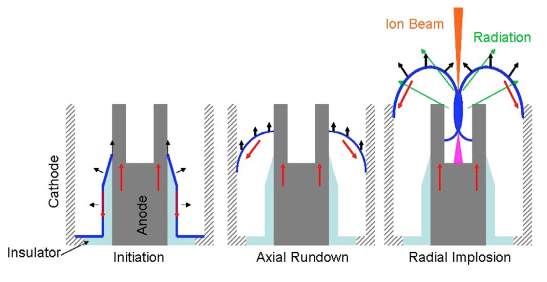
\includegraphics[width=0.7\textwidth]{figures/dfp-phases.png}
        }
        \caption{Three phases of a typical DPF current pulse: initiation via flashover of the insulator, axial run-down phase, and radial implosion of form beams and dense pinch. \cite{krishnan_2012_dense}}
        \label{fig:dfp-phases}
    \end{figure}
\end{frame}

\begin{frame} {X-ray Radiation}
    \begin{itemize}
        \item There are 2 well known mechanisms: line and continuum radiation.
        \item Line radiation: generated by a working gas, or from the interaction between the energetic electrons and impurities.
        \item Continuum radiation: recombination and Bremsstrahlung radiation.
    \end{itemize}
\end{frame}

\begin{frame} {Neutron Emission}
    \begin{itemize}
        \item Two mechanisms: thermal and beam target.
        \item Thermal mechanism: collision of energetic deuterium ions.
        \item Beam target mechanism: interaction of accelerated deuterons with the plasma or background gas.
    \end{itemize}
\end{frame}
\section{Applications}

\begin{frame} {Short-lived Radioisotopes (SLRs) Production}
    \begin{itemize}
        \item SLRs: such as $^{13}$N, $^{17}$F, $^{18}$F, $^{15}$O, and $^{11}$C.
        \item SLRs are used in medical applications.
        \item SLRs production: bombardment of an external solid (exogenous method).
        \item SLRs production: bombardment of a high atomic number gas (endogenous method).
    \end{itemize}
    \begin{figure}
        \centering
        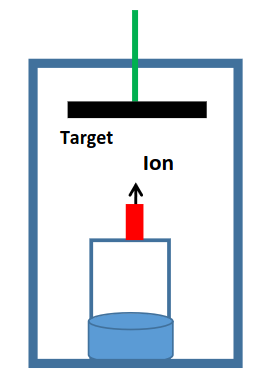
\includegraphics[width=0.2\textwidth]{figures/slr-production.png}
        \caption{The bombardment of target by ion beam generated by plasma.}
        \label{fig:slr-production}
    \end{figure}
\end{frame}

\begin{frame} {Thin Film Deposition}
    \begin{itemize}
        \item Thin film deposition: create thin film coating onto a substrate material.
        \item Electron beam sputters target material.
        \item Sputtered material gets deposited onto the surface of substrate material.
    \end{itemize}
    \begin{figure}
        \centering
        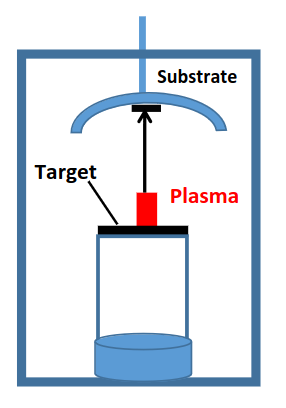
\includegraphics[width=0.2\textwidth]{figures/thin-film-doposition.png}
        \caption{Schematic arrangement for thin film deposition in a plasma focus.}
        \label{fig:thin-film-deposition}
    \end{figure}
\end{frame}

\begin{frame} {Detection of Illicit Materials and Explosives}
    \begin{itemize}
        \item The neutron scattering and the gamma-rays allows us to determine the material.
        \item DFP is a good neutron source.
    \end{itemize}
    \begin{figure}
        \centering
        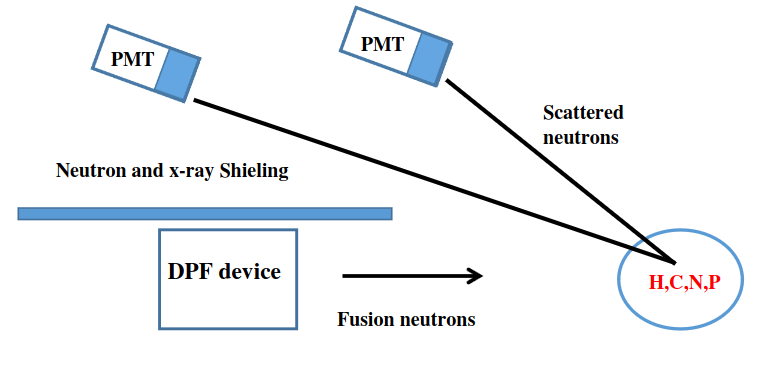
\includegraphics[width=0.7\textwidth]{figures/detection-of-illicit-material.png}
        \caption{Schematic arrangement of illicit and explosive materials detection by a DPF.}
        \label{fig:detection-of-illicit-material}
    \end{figure}
\end{frame}
\section{Lee Model}

\begin{frame} {Lee Model}
    \begin{itemize}
        \item Three phases: break down, axial, and compression phases.
        \item Compression phase: inward shockwave, reflected shockwave, and slow compression phase.
    \end{itemize}
\end{frame}

\begin{frame} {Break Down Phase}
    \begin{itemize}
        \item Gas is ionized, and current layer formed
    \end{itemize}
    \begin{figure}
        \centering
        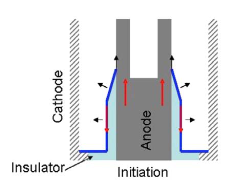
\includegraphics[width=0.5\textwidth]{figures/breakdown-phase.png}
        \caption{Initiation via flashover of the insulator. Break down phase. \cite{krishnan_2012_dense}}
        \label{fig:breakdown-phase}
    \end{figure}
\end{frame}

\begin{frame} {Axial Phase}
    \begin{itemize}
        \item Current layer is accelerated by the $\mathbf{J\times B}$ force in the axial direction.
        \item A shockwave (SW) is formed due to magnetic pressure (MP).
    \end{itemize}
    \begin{figure}
        \centering
        \begin{subfigure}{0.5\textwidth}
            \centering
            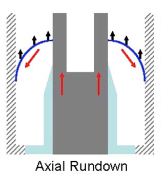
\includegraphics[width=0.5\textwidth]{figures/axial-rundown.png}
            \caption{Axial run-down phase. \cite{krishnan_2012_dense}}
        \end{subfigure}%
        \begin{subfigure}{0.5\textwidth}
            \centering
            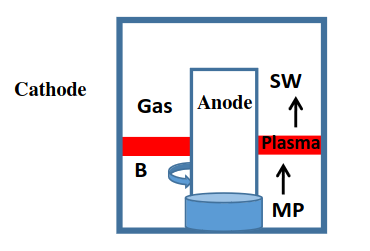
\includegraphics[width=0.7\textwidth]{figures/axial-phase.png}
            \caption{The formation of plasma layer. \cite{behbahani_2017_enhancement}}
        \end{subfigure}
        \label{fig:axial-phase}
    \end{figure}
\end{frame}

\begin{frame} {Compression Phase - Inward Shockwave Phase}
    \begin{itemize}
        \item When the plasma layer arrives at the top of the anode, the $\mathbf{J\times B}$ force pushes them into the center of the anode.
        \item Plasma column with inner radius $r_s$ and outer radius $r_p$ will form on the top of the anode.
        \item Shockwave compresses gas in the center.
    \end{itemize}
    \begin{figure}
        \centering
        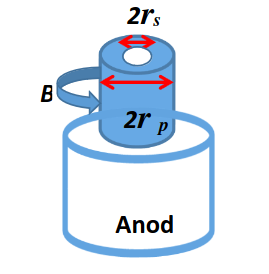
\includegraphics[width=0.4\textwidth]{figures/inward-shockwave-phase.png}
        \caption{The inward radial shock wave in final stage off plasma focus.}
        \label{fig:inward-shockwave-phase}
    \end{figure}
\end{frame}

\begin{frame} {Compression Phase - Reflected Shockwave Phase}
    \begin{itemize}
        \item The shockwave will be reflected radially in the outward direction after hitting the center of the anode.
    \end{itemize}
    \begin{figure}
        \centering
        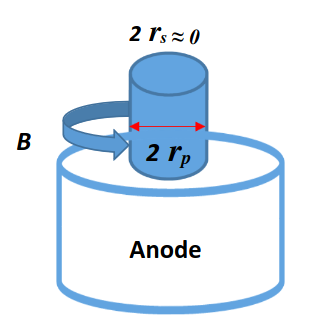
\includegraphics[width=0.4\textwidth]{figures/reflected-shockwave-phase.png}
        \caption{The reflected shockwave phase in plasma focus. \cite{behbahani_2017_enhancement}}
        \label{fig:reflected-shockwave-phase}
    \end{figure}
\end{frame}

\begin{frame} {Compression Phase - Slow Compression Phase}
    \begin{itemize}
        \item Slow compression phase starts when $r_s=r_p$.
        \item The reflected shockwave produces a pressure in the opposite direction of the magnetic pressure.
        \item Plasma column will be compressed to its minimum radius.
    \end{itemize}
\end{frame}

\begin{frame} {Instability Phase}
    \begin{itemize}
        \item When plasma reaches maximum compression, the plasma column may become unstable due to plasma instabilities.
        \item Instabilities make the plasma resistance anomalous.
    \end{itemize}
    \begin{figure}
        \centering
        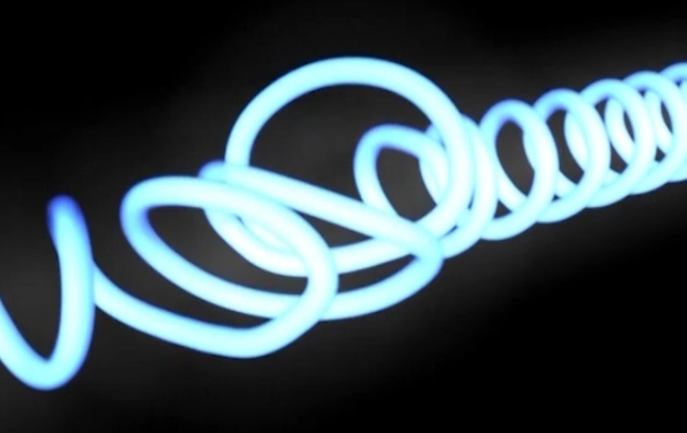
\includegraphics[width=0.7\textwidth]{figures/instability-phase.png}
        \caption{Plasma column is twisted in instability phase. Source \cite{lppfusion_device_fusion}}
        \label{fig:instability-phase}
    \end{figure}
\end{frame}

%%%%%%%%%%%%%%%%%%%%
% references
%%%%%%%%%%%%%%%%%%%%
\newpage
\begin{frame}[allowframebreaks]
	\bibliographystyle{abbrv}
	\bibliography{../references}
	\nocite{*}
\end{frame}

\end{document}
